\documentclass[tikz,border=5pt]{standalone}

\usepackage{lmodern}
\usepackage{amsmath,amssymb}
\usetikzlibrary{
  arrows.meta,
  calc,
  decorations.pathmorphing,
  positioning,
  shadings
}

\definecolor{Ink}{HTML}{1E2830}
\definecolor{Muted}{HTML}{66727C}
\definecolor{ArrowGray}{HTML}{C2C7CB}
\definecolor{BoxGray}{HTML}{B8C0C6}
\definecolor{Navy}{HTML}{123B73}
\definecolor{PaleBlue}{HTML}{C7DDF4}
\definecolor{SurfaceBlue}{HTML}{DCEAF5}
\definecolor{Orange}{HTML}{E56F00}
\definecolor{OrangeDark}{HTML}{9F4C00}
\definecolor{LocalBlue}{HTML}{1663AD}
\definecolor{FinalGreen}{HTML}{12604F}

\tikzset{
  flowarrow/.style={-{Latex[length=3.2mm,width=2.6mm]},draw=ArrowGray,line width=2.2pt},
  panelorange/.style={draw=Orange,line width=.75pt,rounded corners=5pt,fill=white},
  panelblue/.style={draw=LocalBlue,line width=.75pt,rounded corners=5pt,fill=white},
  panelfinal/.style={draw=FinalGreen,line width=.9pt,rounded corners=5pt,fill=FinalGreen!3},
  boxline/.style={draw=BoxGray,line width=.45pt},
  hidden/.style={draw=Navy!55,dashed,line width=.45pt},
  hydro/.style={draw=Navy,line width=.8pt,fill=PaleBlue,fill opacity=.68},
  graphline/.style={draw=Ink!78,line width=.5pt},
  missingline/.style={draw=Ink!72,dashed,line width=.55pt},
  tinybranch/.style={draw=Navy!55,line width=.3pt},
}

\newcommand{\ballnode}[3]{%
  \shade[ball color=#3,draw=Ink!72,line width=.25pt] #1 circle (#2);%
}

\newcommand{\wirebox}{%
  \draw[boxline] (-.55,-.72) rectangle (.55,.50);
  \draw[boxline] (-.26,-.50) rectangle (.84,.72);
  \draw[boxline] (-.55,-.72)--(-.26,-.50)
                 (.55,-.72)--(.84,-.50)
                 (.55,.50)--(.84,.72)
                 (-.55,.50)--(-.26,.72);
}

\newcommand{\hydrotriangle}[2]{%
  \begin{scope}[shift={#1},scale=#2]
    \wirebox
    \path[hydro] (-.48,-.62)--(.48,-.62)--(-.08,.30)--cycle;
    \draw[hidden] (-.48,-.62)--(-.08,.30);
  \end{scope}
}

\newcommand{\hydrotrapezoid}[2]{%
  \begin{scope}[shift={#1},scale=#2]
    \wirebox
    \path[hydro] (-.50,-.62)--(.50,-.62)--(.25,.34)--(-.13,.54)--cycle;
    \draw[hidden] (-.13,.54)--(.25,.34);
  \end{scope}
}

\newcommand{\hydropentagon}[2]{%
  \begin{scope}[shift={#1},scale=#2]
    \wirebox
    \path[hydro] (-.48,-.28)--(-.17,.52)--(.27,.36)--(.49,-.22)--(.10,-.64)--cycle;
    \draw[hidden] (-.48,-.28)--(.27,.36);
  \end{scope}
}

\newcommand{\hydroparallelogram}[2]{%
  \begin{scope}[shift={#1},scale=#2]
    \wirebox
    \path[hydro] (-.42,-.55)--(-.42,.38)--(.20,.56)--(.49,-.36)--cycle;
    \draw[hidden] (-.42,.38)--(.49,-.36);
  \end{scope}
}

\newcommand{\bighydro}[2]{%
  \begin{scope}[shift={#1},scale=#2]
    \draw[boxline] (-1.10,-.95) rectangle (.75,.82);
    \draw[boxline] (-.58,-.55) rectangle (1.27,1.22);
    \draw[boxline] (-1.10,-.95)--(-.58,-.55)
                   (.75,-.95)--(1.27,-.55)
                   (.75,.82)--(1.27,1.22)
                   (-1.10,.82)--(-.58,1.22);
    \path[draw=Navy,line width=.8pt,fill=PaleBlue,fill opacity=.55]
      (-1.00,-.55)--(-.63,.77)--(-.12,1.05)--(.86,.76)--(1.12,.02)--
      (.62,-.78)--(-.14,-.96)--cycle;
    \path[draw=Navy!88,line width=.7pt,fill=PaleBlue!80!white,fill opacity=.43]
      (-1.00,-.55)--(-.12,1.05)--(.24,.20)--(-.14,-.96)--cycle;
    \path[draw=Navy!88,line width=.7pt,fill=PaleBlue!65!white,fill opacity=.38]
      (-.12,1.05)--(.86,.76)--(1.12,.02)--(.24,.20)--cycle;
    \draw[hidden] (-.63,.77)--(.24,.20)--(.62,-.78);
    \draw[hidden] (-1.00,-.55)--(.24,.20)--(1.12,.02);
  \end{scope}
}

\begin{document}
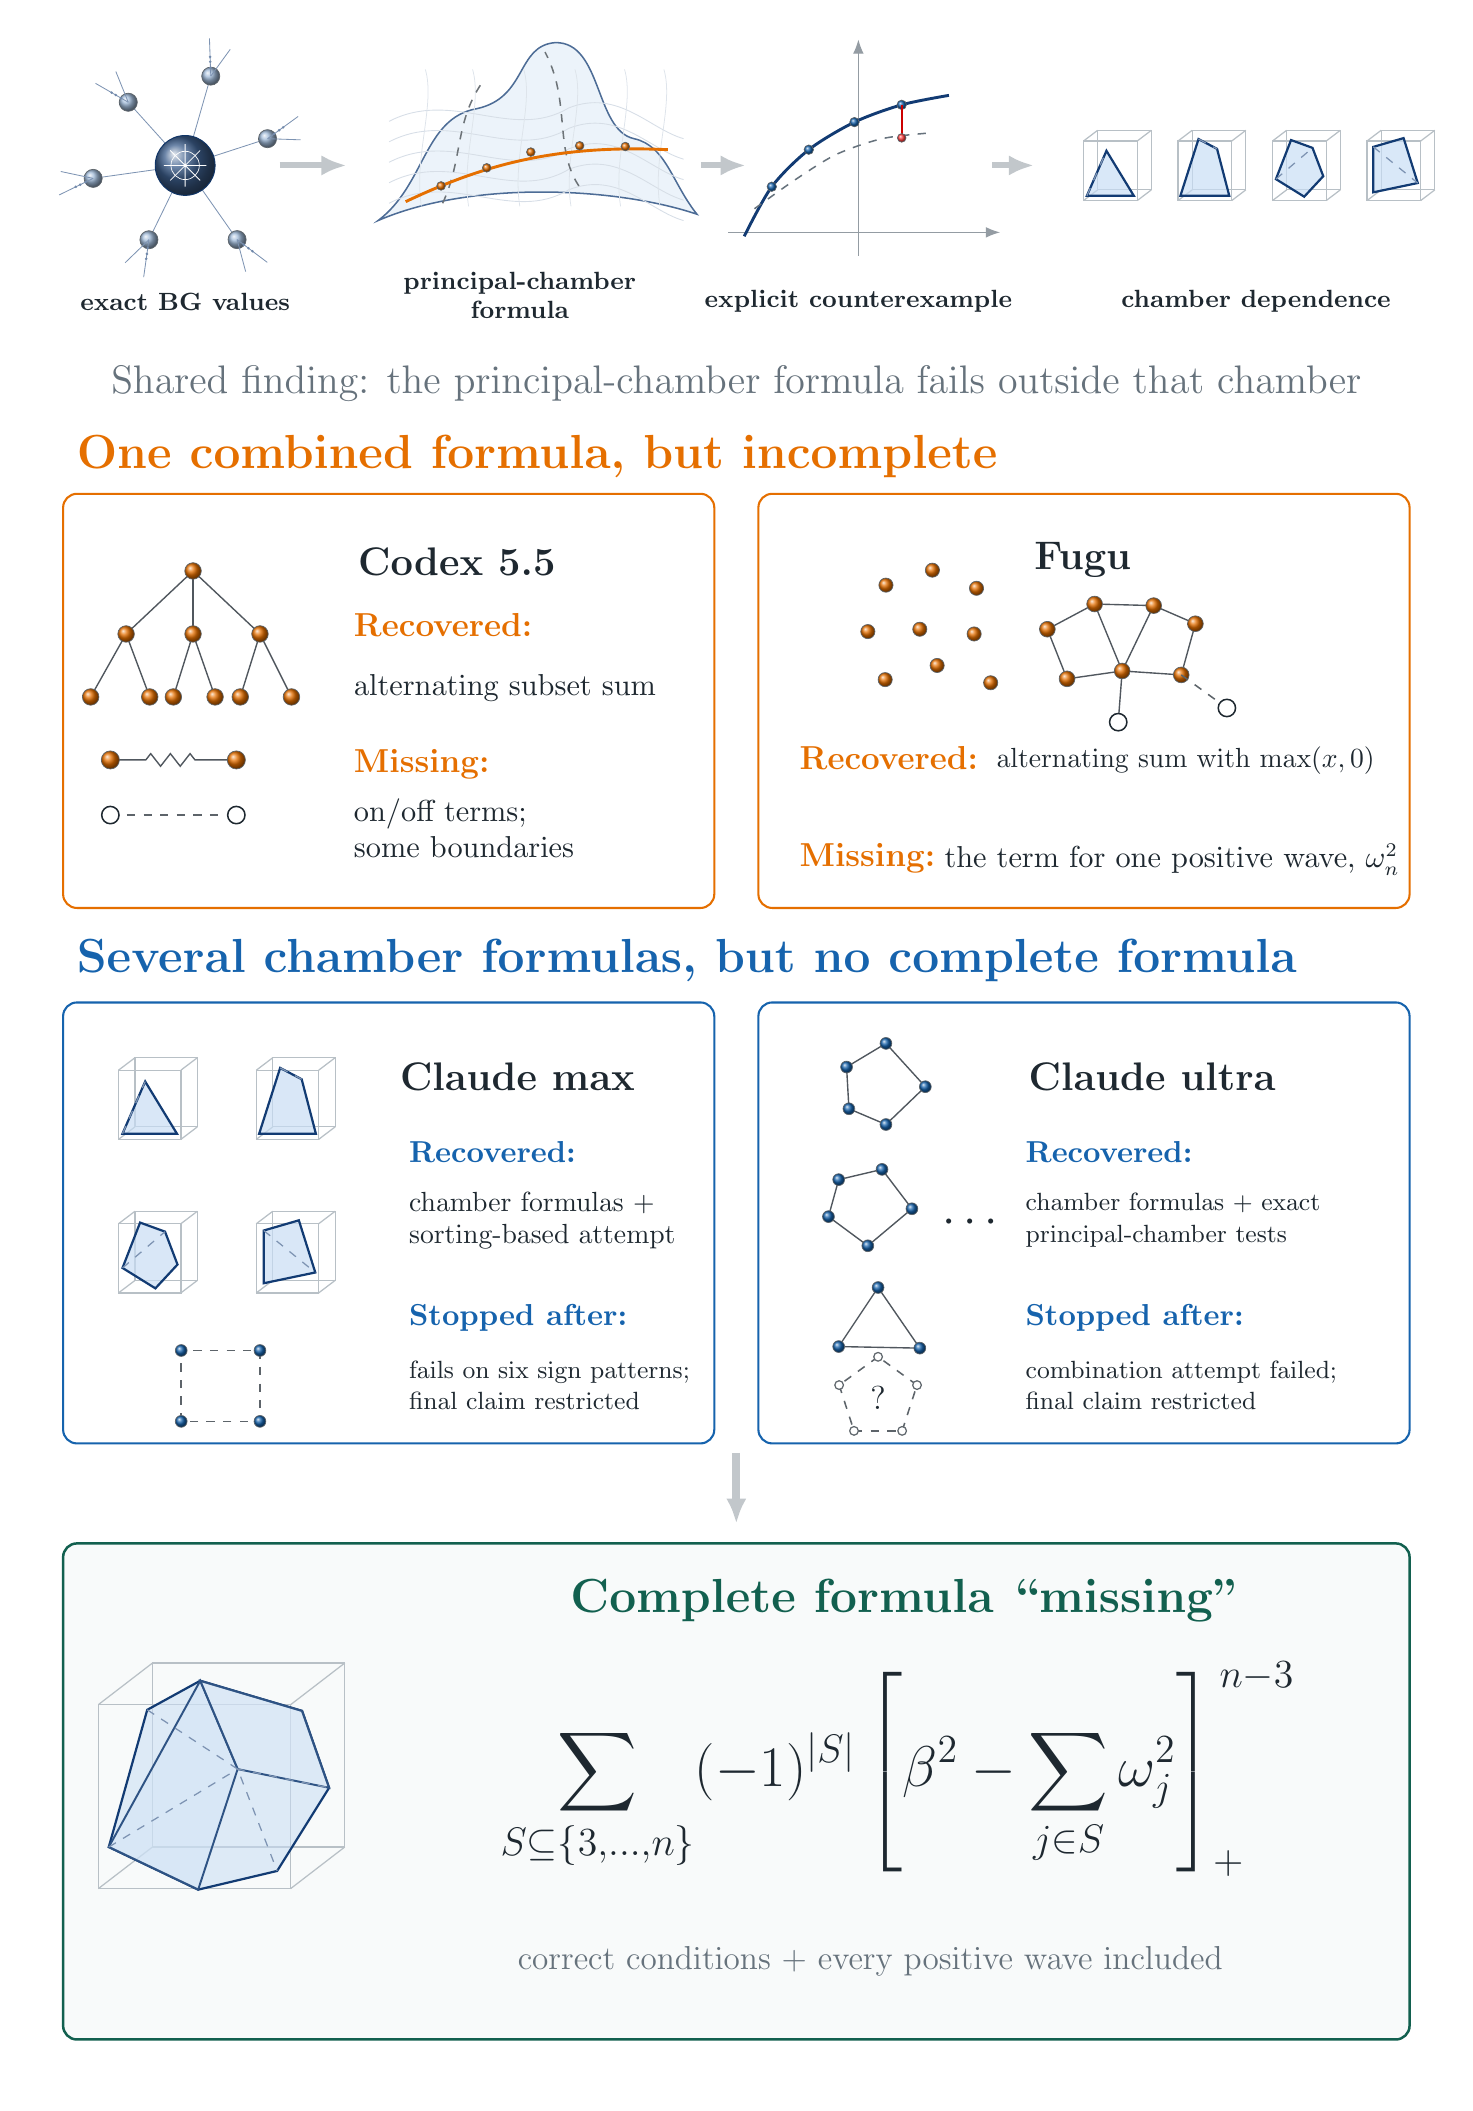
\begin{tikzpicture}[x=1cm,y=1cm]
  \path[use as bounding box] (0,0) rectangle (18,26.1);

  % ---------------------------------------------------------------------------
  % Common discovery path: oracle
  % ---------------------------------------------------------------------------
  \begin{scope}[shift={(2.0,24.35)}]
    \foreach \a/\r in {18/1.10,74/1.18,132/1.08,188/1.18,244/1.05,305/1.15}{
      \draw[tinybranch] (0,0)--(\a:\r);
      \ballnode{(\a:\r)}{.115}{PaleBlue!78!Navy}
    }
    \foreach \a/\r/\b in {18/1.10/7,74/1.18/19,132/1.08/12,188/1.18/17,244/1.05/10,305/1.15/15}{
      \draw[tinybranch] (\a:\r)--($(\a:\r)+(\a+18:.48)$);
      \draw[tinybranch] (\a:\r)--($(\a:\r)+(\a-20:.42)$);
      \foreach \t in {.22,.38,.51}{
        \fill[Navy!60] ($(\a:\r)!\t!($(\a:\r)+(\a+18:.48)$)$) circle (.018);
      }
    }
    \shade[ball color=Navy!82,draw=Navy!90!black,line width=.35pt] (0,0) circle (.38);
    \draw[white!75,line width=.3pt] (-.27,0)--(.27,0) (0,-.27)--(0,.27)
      (-.19,-.19)--(.19,.19) (-.19,.19)--(.19,-.19);
    \draw[white!55,line width=.25pt] (0,0) circle (.18);
  \end{scope}

  % Principal-chamber surface
  \begin{scope}[shift={(6.45,24.35)}]
    \path[fill=SurfaceBlue,fill opacity=.55,draw=Navy!75,line width=.55pt]
      (-2.00,-.70) .. controls (-1.40,-.25) and (-1.42,.60) .. (-.75,.72)
      .. controls (-.10,.86) and (-.25,1.52) .. (.25,1.56)
      .. controls (.85,1.57) and (.75,.45) .. (1.25,.34)
      .. controls (1.66,.25) and (1.73,-.22) .. (2.05,-.62)
      .. controls (1.05,-.28) and (-.80,-.18) .. (-2.00,-.70)--cycle;
    \foreach \yy in {-.48,-.22,.04,.30,.56}{
      \draw[Navy!17,line width=.32pt]
        (-1.86,\yy) .. controls (-1.05,\yy+.42) and (-.30,\yy-.26) .. (.42,\yy+.17)
        .. controls (1.05,\yy+.42) and (1.45,\yy-.10) .. (1.88,\yy-.22);
    }
    \foreach \xx in {-1.45,-.85,-.20,.45,1.08,1.58}{
      \draw[Navy!14,line width=.28pt]
        (\xx,-.52) .. controls (\xx-.10,.10) and (\xx+.18,.78) .. (\xx+.05,1.22);
    }
    \draw[Ink!65,dashed,line width=.55pt]
      (-1.18,-.48) .. controls (-.92,.08) and (-1.03,.54) .. (-.68,1.05);
    \draw[Ink!65,dashed,line width=.55pt]
      (.55,-.26) .. controls (.23,.22) and (.45,.82) .. (.12,1.44);
    \draw[Orange,line width=1.05pt]
      (-1.65,-.46) .. controls (-.72,-.02) and (.20,.27) .. (1.68,.20);
    \foreach \p in {(-1.20,-.26),(-.62,-.03),(-.06,.17),(.56,.25),(1.14,.24)}{
      \ballnode{\p}{.055}{Orange}
    }
  \end{scope}

  % Explicit counterexample
  \begin{scope}[shift={(10.55,24.30)}]
    \draw[-{Latex[length=1.8mm]},draw=Muted!70,line width=.45pt] (-1.65,-.80)--(1.80,-.80);
    \draw[-{Latex[length=1.8mm]},draw=Muted!70,line width=.45pt] (0,-1.10)--(0,1.65);
    \draw[Navy,line width=1.05pt]
      plot[smooth] coordinates {(-1.45,-.85) (-1.10,-.22) (-.63,.25) (-.05,.60) (.55,.82) (1.15,.94)};
    \draw[Muted,dashed,line width=.55pt]
      plot[smooth] coordinates {(-1.32,-.50) (-.80,-.13) (-.28,.19) (.30,.39) (.88,.46)};
    \foreach \p in {(-1.10,-.22),(-.63,.25),(-.05,.60),(.55,.82)}{
      \ballnode{\p}{.060}{LocalBlue}
    }
    \draw[red!80!black,line width=.8pt] (.55,.82)--(.55,.40);
    \ballnode{(.55,.40)}{.055}{red!75}
  \end{scope}

  % Piecewise hydrotope cross-sections
  \hydrotriangle{(13.75,24.35)}{.62}
  \hydrotrapezoid{(14.95,24.35)}{.62}
  \hydropentagon{(16.15,24.35)}{.62}
  \hydroparallelogram{(17.35,24.35)}{.62}

  % Flow arrows between the four stages
  \draw[flowarrow] (3.20,24.35)--(4.05,24.35);
  \draw[flowarrow] (8.55,24.35)--(9.12,24.35);
  \draw[flowarrow] (12.25,24.35)--(12.78,24.35);

  % Stage labels
  \node[font=\fontsize{9.2}{10.5}\selectfont\bfseries,text=Ink] at (2.0,22.62) {exact BG values};
  \node[align=center,font=\fontsize{9.2}{10.5}\selectfont\bfseries,text=Ink]
    at (6.25,22.70) {principal-chamber\\formula};
  \node[font=\fontsize{9.2}{10.5}\selectfont\bfseries,text=Ink] at (10.55,22.62) {explicit counterexample};
  \node[font=\fontsize{9.2}{10.5}\selectfont\bfseries,text=Ink] at (15.60,22.62) {chamber dependence};
  \node[font=\fontsize{14}{16}\selectfont,text=Muted] at (9.0,21.58)
    {Shared finding: the principal-chamber formula fails outside that chamber};

  % ---------------------------------------------------------------------------
  % Incomplete combined formulas
  % ---------------------------------------------------------------------------
  \node[anchor=west,font=\fontsize{16}{18}\selectfont\bfseries,text=Orange] at (.50,20.65)
    {One combined formula, but incomplete};
  \draw[panelorange] (.45,14.92) rectangle (8.72,20.18);
  \draw[panelorange] (9.28,14.92) rectangle (17.55,20.18);

  % Codex 5.5: alternating tree / incomplete links
  \begin{scope}[shift={(2.10,17.55)}]
    \coordinate (r) at (0,1.65);
    \coordinate (a) at (-.85,.85); \coordinate (b) at (0,.85); \coordinate (c) at (.85,.85);
    \coordinate (a1) at (-1.30,.05); \coordinate (a2) at (-.55,.05);
    \coordinate (b1) at (-.25,.05); \coordinate (b2) at (.28,.05);
    \coordinate (c1) at (.60,.05); \coordinate (c2) at (1.25,.05);
    \foreach \u/\v in {r/a,r/b,r/c,a/a1,a/a2,b/b1,b/b2,c/c1,c/c2}{
      \draw[graphline] (\u)--(\v);
    }
    \foreach \p in {r,a,b,c,a1,a2,b1,b2,c1,c2}{
      \ballnode{(\p)}{.105}{Orange}
    }
    \draw[graphline] (-1.05,-.75)--(-.60,-.75)
      decorate[decoration={zigzag,segment length=2.5mm,amplitude=.8mm}]{--(.10,-.75)}--(.55,-.75);
    \ballnode{(-1.05,-.75)}{.115}{Orange}
    \ballnode{(.55,-.75)}{.115}{Orange}
    \draw[missingline] (-1.05,-1.45)--(.55,-1.45);
    \draw[Ink,line width=.55pt,fill=white] (-1.05,-1.45) circle (.11);
    \draw[Ink,line width=.55pt,fill=white] (.55,-1.45) circle (.11);
  \end{scope}
  \node[font=\fontsize{15}{17}\selectfont\bfseries,text=Ink] at (5.45,19.32) {Codex 5.5};
  \node[anchor=west,font=\fontsize{11.5}{13}\selectfont\bfseries,text=Orange] at (4.02,18.52) {Recovered:};
  \node[anchor=west,align=left,font=\fontsize{10.8}{13}\selectfont,text=Ink] at (4.02,17.72)
    {alternating subset sum};
  \node[anchor=west,font=\fontsize{11.5}{13}\selectfont\bfseries,text=Orange] at (4.02,16.75) {Missing:};
  \node[anchor=west,align=left,font=\fontsize{10.8}{13}\selectfont,text=Ink] at (4.02,15.94)
    {on/off terms;\\some boundaries};

  % Fugu: scattered parts, nearly assembled graph, one open connection
  \begin{scope}[shift={(12.95,18.28)}]
    \foreach \p in {(-2.05,.74),(-1.46,.93),(-.90,.70),(-2.28,.15),(-1.62,.18),(-.93,.12),(-2.06,-.46),(-1.40,-.28),(-.72,-.50)}{
      \ballnode{\p}{.09}{Orange}
    }
    \coordinate (g1) at (.00,.18); \coordinate (g2) at (.60,.50); \coordinate (g3) at (1.35,.48);
    \coordinate (g4) at (.25,-.45); \coordinate (g5) at (.95,-.35); \coordinate (g6) at (1.70,-.40);
    \coordinate (g7) at (.90,-1.00); \coordinate (g8) at (1.88,.25);
    \foreach \u/\v in {g1/g2,g2/g3,g1/g4,g2/g5,g3/g5,g4/g5,g5/g6,g5/g7,g6/g8,g3/g8}{
      \draw[graphline] (\u)--(\v);
    }
    \foreach \p in {g1,g2,g3,g4,g5,g6,g8}{
      \ballnode{(\p)}{.10}{Orange}
    }
    \draw[Ink,line width=.55pt,fill=white] (g7) circle (.11);
    \draw[missingline] (g6)--(2.28,-.82);
    \draw[Ink,line width=.55pt,fill=white] (2.28,-.82) circle (.11);
  \end{scope}
  \node[font=\fontsize{15}{17}\selectfont\bfseries,text=Ink] at (13.40,19.34) {Fugu};
  \node[anchor=west,font=\fontsize{11.5}{13}\selectfont\bfseries,text=Orange] at (9.68,16.82) {Recovered:};
  \node[anchor=west,font=\fontsize{9.7}{12}\selectfont,text=Ink] at (12.18,16.79)
    {alternating sum with $\max(x,0)$};
  \node[anchor=west,font=\fontsize{11.5}{13}\selectfont\bfseries,text=Orange] at (9.68,15.55) {Missing:};
  \node[anchor=west,font=\fontsize{10.5}{13}\selectfont,text=Ink] at (11.52,15.53)
    {the term for one positive wave, $\omega_n^2$};

  % ---------------------------------------------------------------------------
  % Separate chamber formulas
  % ---------------------------------------------------------------------------
  \node[anchor=west,font=\fontsize{16}{18}\selectfont\bfseries,text=LocalBlue] at (.50,14.25)
    {Several chamber formulas, but no complete formula};
  \draw[panelblue] (.45,8.12) rectangle (8.72,13.72);
  \draw[panelblue] (9.28,8.12) rectangle (17.55,13.72);

  % Claude max: four hydrotope chamber sections
  \hydrotriangle{(1.55,12.50)}{.72}
  \hydrotrapezoid{(3.30,12.50)}{.72}
  \hydropentagon{(1.55,10.55)}{.72}
  \hydroparallelogram{(3.30,10.55)}{.72}
  \begin{scope}[shift={(2.45,8.85)}]
    \draw[missingline] (-.50,-.45) rectangle (.50,.45);
    \ballnode{(-.50,-.45)}{.075}{LocalBlue}
    \ballnode{(.50,-.45)}{.075}{LocalBlue}
    \ballnode{(-.50,.45)}{.075}{LocalBlue}
    \ballnode{(.50,.45)}{.075}{LocalBlue}
  \end{scope}
  \node[font=\fontsize{15}{17}\selectfont\bfseries,text=Ink] at (6.22,12.78) {Claude max};
  \node[anchor=west,font=\fontsize{11.2}{13}\selectfont\bfseries,text=LocalBlue] at (4.72,11.82) {Recovered:};
  \node[anchor=west,align=left,font=\fontsize{9.7}{11.8}\selectfont,text=Ink] at (4.72,10.95)
    {chamber formulas +\\sorting-based attempt};
  \node[anchor=west,font=\fontsize{11.2}{13}\selectfont\bfseries,text=LocalBlue] at (4.72,9.72) {Stopped after:};
  \node[anchor=west,align=left,font=\fontsize{9.3}{11.4}\selectfont,text=Ink] at (4.72,8.86)
    {fails on six sign patterns;\\final claim restricted};

  % Claude ultra: several chamber graphs and no combined formula
  \begin{scope}[shift={(10.85,12.55)}]
    \coordinate (u1) at (-.45,.35); \coordinate (u2) at (.05,.65);
    \coordinate (u3) at (.55,.10); \coordinate (u4) at (.05,-.38); \coordinate (u5) at (-.42,-.18);
    \foreach \a/\b in {u1/u2,u2/u3,u3/u4,u4/u5,u5/u1}{
      \draw[graphline] (\a)--(\b);
    }
    \foreach \p in {u1,u2,u3,u4,u5}{\ballnode{(\p)}{.075}{LocalBlue}}
  \end{scope}
  \begin{scope}[shift={(10.75,11.05)}]
    \coordinate (v1) at (-.45,.42); \coordinate (v2) at (.10,.55);
    \coordinate (v3) at (.48,.05); \coordinate (v4) at (-.08,-.42); \coordinate (v5) at (-.58,-.05);
    \foreach \a/\b in {v1/v2,v2/v3,v3/v4,v4/v5,v5/v1}{
      \draw[graphline] (\a)--(\b);
    }
    \foreach \p in {v1,v2,v3,v4,v5}{\ballnode{(\p)}{.075}{LocalBlue}}
  \end{scope}
  \begin{scope}[shift={(10.75,9.65)}]
    \coordinate (w1) at (-.45,-.30); \coordinate (w2) at (.05,.45); \coordinate (w3) at (.58,-.32);
    \foreach \a/\b in {w1/w2,w2/w3,w3/w1}{\draw[graphline] (\a)--(\b);}
    \foreach \p in {w1,w2,w3}{\ballnode{(\p)}{.075}{LocalBlue}}
  \end{scope}
  \node[font=\fontsize{17}{18}\selectfont,text=Ink] at (12.02,10.92) {$\cdots$};
  \begin{scope}[shift={(10.80,8.70)}]
    \foreach \i in {0,...,4}{
      \coordinate (q\i) at ({90+72*\i}:.52);
    }
    \foreach \i [evaluate=\i as \j using {int(mod(\i+1,5))}] in {0,...,4}{
      \draw[missingline] (q\i)--(q\j);
    }
    \foreach \p in {q0,q1,q2,q3,q4}{
      \draw[Ink!70,line width=.45pt,fill=white] (\p) circle (.055);
    }
    \node[font=\fontsize{12}{12}\selectfont,text=Ink] at (0,0) {?};
  \end{scope}
  \node[font=\fontsize{15}{17}\selectfont\bfseries,text=Ink] at (14.28,12.78) {Claude ultra};
  \node[anchor=west,font=\fontsize{11.2}{13}\selectfont\bfseries,text=LocalBlue] at (12.55,11.82) {Recovered:};
  \node[anchor=west,align=left,font=\fontsize{9.5}{11.6}\selectfont,text=Ink] at (12.55,10.95)
    {chamber formulas + exact\\principal-chamber tests};
  \node[anchor=west,font=\fontsize{11.2}{13}\selectfont\bfseries,text=LocalBlue] at (12.55,9.72) {Stopped after:};
  \node[anchor=west,align=left,font=\fontsize{9.1}{11.2}\selectfont,text=Ink] at (12.55,8.86)
    {combination attempt failed;\\final claim restricted};

  % ---------------------------------------------------------------------------
  % Complete formula
  % ---------------------------------------------------------------------------
  \draw[flowarrow,line width=3.0pt] (9.00,8.00)--(9.00,7.10);
  \draw[panelfinal] (.45,.55) rectangle (17.55,6.85);
  \bighydro{(2.35,3.72)}{1.32}
  \node[font=\fontsize{16}{18}\selectfont\bfseries,text=FinalGreen] at (11.15,6.12)
    {Complete formula ``missing"};
  \node[font=\fontsize{20}{24}\selectfont,text=Ink] at (11.05,3.98)
    {$\displaystyle
      \sum_{S\subseteq\{3,\ldots,n\}}(-1)^{|S|}
      \left[\beta^2-\sum_{j\in S}\omega_j^2\right]_{+}^{\,n-3}$};
  \node[font=\fontsize{12.5}{15}\selectfont,text=Muted] at (10.70,1.55)
    {correct conditions + every positive wave included};

\end{tikzpicture}
\end{document}
